
\begin{table}[tbp] 
\setlength{\abovecaptionskip}{-1pt}
\setlength{\belowcaptionskip}{-10pt}
\caption{Simulator details.}
\begin{center}
\renewcommand\arraystretch{1.2}
\resizebox{\linewidth}{!}{
\begin{tabular}{c|c|c|c}
\toprule
\multicolumn{2}{c|}{\textbf{GPU Configuration}} & \multicolumn{2}{c}{\textbf{ACC Configuration}} \\
\hline
\textbf{Processor} & 8 A100 & \textbf{CPU} & 2TB + 406GB/s \\
\hline
\textbf{Capacity} & 640GB & \textbf{HBM-PIM} & \makecell[c]{640GB + 260.8TB/s (GPU-side) \\ \REVISE{320GB + 130.4TB/s (Extended)}}\\
\hline
\textbf{Bandwidth} & 16.3TB/s& \textbf{DIMM-PIM} & \makecell[c]{2TB + 1.6TB/s (R-PIM) \\ 2TB + 13.0TB/s (\sys)}\\
\hline
\multicolumn{4}{c}{\textbf{DIMM / DIMM-PIM: DDR4-3200}} \\
\hline
\textbf{Hierarchy} &  \multicolumn{3}{c}{ 2 Ranks (8 Chips) $\times$ 4 Bank Groups $\times$ 4 Banks}\\
\hline
\textbf{DRAM Timing} &
\multicolumn{3}{c}{\makecell[c]{BL=4:CCD=4:RRD=4/8:RCD=22:RAS=52:RP=22:RC=74:\\CL=22:WL=16:CDLR=4/12:WR=24:CCDL=8:RTP=12}} \\
\bottomrule


\multicolumn{4}{l}{ * Bank PU's compute-memory ratio $N_{cmr}$=n for GQA-n.} \\

\end{tabular}}
\label{tab:simulator}
\end{center}
\end{table}

\begin{table}[tbp]
\setlength{\abovecaptionskip}{-1pt}
\setlength{\belowcaptionskip}{-10pt}
\caption{The evaluated LLM models.}
\begin{center}
\renewcommand\arraystretch{1.2}
\resizebox{\linewidth}{!}{
\begin{tabular}{c|cccc|cc}

\toprule

\textbf{Model} & \textbf{Layers} $\mathbf{N_l}$ & \textbf{Heads} $\mathbf{N_{h}}$ & \textbf{Embedding} $\mathbf{D_e}$ & \textbf{Type} & \textbf{TP} & \textbf{DP} \\

\hline

\textbf{OPT-66B} & 64 & 72 & 9216 & MHA & 2 & 4 \\
\hline

\textbf{QWEN-72B} & 80 & 64 & 8192 & GQA-8  & 4  & 2 \\

\hline

\textbf{GPT-175B} & 96 & 96 & 12288 & MHA  & 8  & 1  \\
\bottomrule


\multicolumn{7}{l}{ * Precision: FP16; Head Embedding: $E_{h} = D_{e}/N_{h}=128$.} \\

\end{tabular}}

\label{tab:model}
\end{center}
\end{table}

\begin{table}[t]
    \setlength{\abovecaptionskip}{-1pt}
    \setlength{\belowcaptionskip}{-10pt}
    \caption{Real-world traces.}
    \begin{center}
    \renewcommand\arraystretch{1.2}
    \resizebox{\linewidth}{!}{
        \begin{tabular}{c|cccc}
            \toprule
            \textbf{Trace}           & \makecell[c]{\textbf{Avg.} $\mathbf{L_{in}}$}& \makecell[c]{\textbf{Std.} $\mathbf{L_{in}}$}  & \makecell[c]{\textbf{Avg.} $\mathbf{L_{out}}$}  & \makecell[c]{\textbf{Std.} $\mathbf{L_{out}}$} \\ 
            \hline
            \textbf{OpenR1-Math-220k}~\cite{open-r1} & 96.0              & 75.1              & 12684.1            & 8464.6             \\ 
            \hline
            \textbf{Dolphin-r1}~\cite{dophin}       & 201.9              & 563.0              & 3926.2            & 4216.0             \\ 
            \hline
            \textbf{OpenThoughts-114k-math}~\cite{OpenThoughts-114k-math} & 89.4              & 66.7              & 6366.7            & 4662.9             \\ 
            \bottomrule
            \end{tabular}
    }
    
    \label{tab:traces}
    \end{center}
    \end{table}


\section{Evaluation}
\label{sec:eval}
\begin{figure*}[htb]
  \setlength{\belowcaptionskip}{-5pt}
  \begin{minipage}[t]{0.24\linewidth}
      \centering
      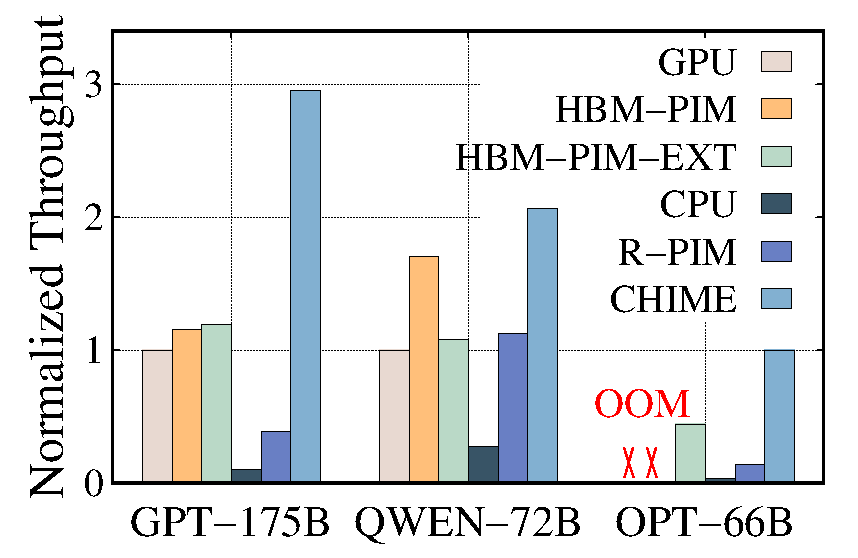
\includegraphics[width=\textwidth]{figs-eval/eval-end-to-end-throughput1.eps}
      \footnotesize
      \textbf{(a) OpenR1.}
\end{minipage}
\begin{minipage}[t]{0.24\linewidth}
  \centering
  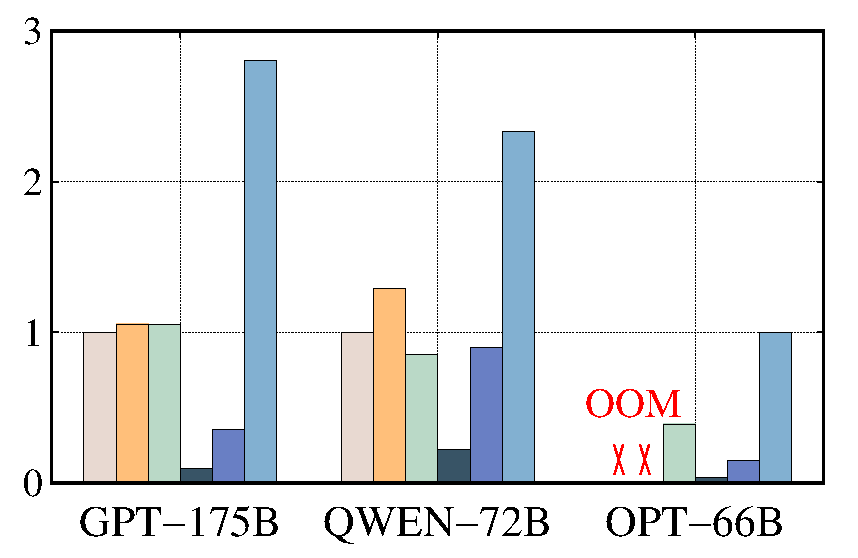
\includegraphics[width=\textwidth]{figs-eval/eval-end-to-end-throughput3.eps}
  \footnotesize
  \textbf{(b) OpenThoughts.}
\end{minipage}
\begin{minipage}[t]{0.24\linewidth}
  \centering
  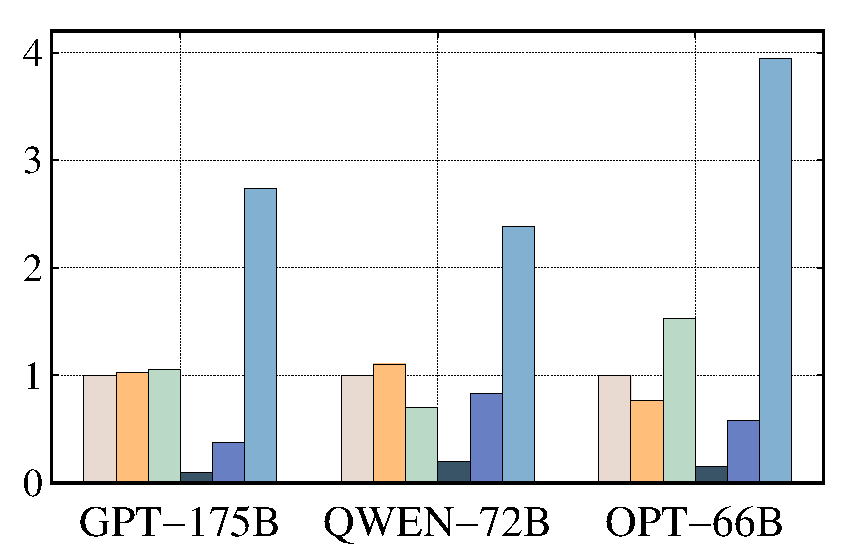
\includegraphics[width=\textwidth]{figs-eval/eval-end-to-end-throughput2.eps}
  \footnotesize
  \textbf{(c) Dolphin.}
\end{minipage}
\begin{minipage}[t]{0.24\linewidth}
  \centering
  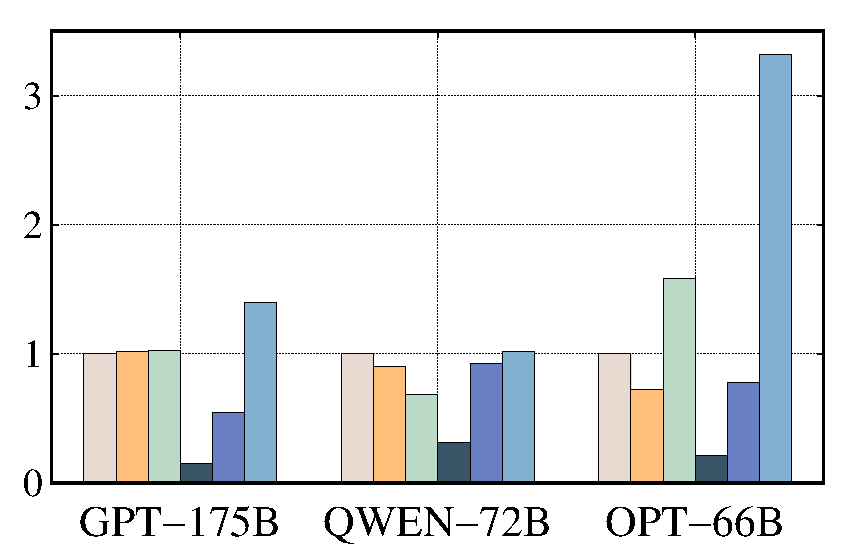
\includegraphics[width=\textwidth]{figs-eval/eval-end-to-end-throughput-short.eps}
  \footnotesize
  \textbf{\REVISE{(d) Dolphin-short.}}
\end{minipage}
\caption{\textbf{End-to-end inference throughput on real-world traces.} \normalfont{\textit{The throughput of GPU-only baseline is normalized to 1. 
For the OPT-66B model, GPU out-of-memory (OOM) errors occurred in two traces, so the throughput of \sys is normalized to 1. 
In case (d), length of requests is reduced by 10$\times$.}}}
  \label{figs:eval-end-to-end-throughput}
\end{figure*}

\subsection{Methodology}
\label{sec:eval-setup}
\myparagraph{Experimental setup.}
Following prior works~\cite{cao2025moelightening,heo2024neupims,sheng2023flexgen}, our goal is achieving \emph{high inference throughput} in the long-context and decoding-dominant scenario.
The evaluation is built upon DGX-A100~\cite{nv2023dgxa100}.
On the GPU side, 8 NVIDIA A100 GPUs, each with 5 HBM2e of 80 GB capacity, are integrated, providing a total of 156 TFLOPs on FP16.
The GPUs are connected via NVLink~\cite{wei2023nvlink}.
On the CPU side, there are 16 channels with 2 DIMMs of total 2TB capacity, equipped with the proposed PIM. 
We develop a simulator integrating
(1) AttAcc~\cite{park2024attacc}, the roofline-based simulation for GPU;
and (2) \sys-PIM-sim based on modified DRAMSim3~\cite{li2020dramsim3}, the trace-driven simulation for \sys-PIM.
\REVISE{We add PIM commands, related timing constraints, and FIFO-based scheduling methods for cycle-level simulation.}






\myparagraph{Baseline systems.}
We compare \sys with one GPU baseline and four AFD baseline systems: 
(1) \emph{GPU-only}, which executes LLM inference exclusively on GPUs. 
(2) \emph{GPU with HBM-PIM}, which equips all existing GPU HBMs with bank-level PUs.
\REVISE{(3) \emph{GPU with HBM-PIM-EXT}, which equips with extended disaggregated HBM-PIMs.
Compared to the ``HBM-PIM'' baseline, the HBM-PIMs in ``HBM-PIM-EXT'' do not store model parameters.}
(4) \emph{GPU with rank-level DIMM-PIM} (R-PIM), which equips all DIMMs with rank-level PUs.
(5) \emph{GPU with CPU offloading}, which leverages CPU as the accelerator.
Our simulations of baseline systems uniformly assume maximal accelerator-side bandwidth utilization during attention computation.
Table~\ref{tab:simulator} lists the hardware specifications. 
\REVISE{For GPU, CPU, and DIMM(-PIM) configurations, we follow the configurations in DGX-A100 systems. 
For HBM-PIM-EXT, considering that HBM2e is more than $6\times$ the price of DDR4~\cite{cost-ddr5-hbm, cost-ddr4,cost-ddr5}, we configure 20 HBM-PIM modules (320\,GB) to provide $\sim$$1/6$ of the capacity available in \sys.
}




\myparagraph{LLM models.}
We evaluate \sys on three LLM models with varying model sizes: OPT-66B, QWEN-72B, and GPT-175B, with FP16 as the data precision.
Considering both the GPU memory capacity and inter-GPU communication overhead, we apply various parallelism configurations, listed in Table~\ref{tab:model}.

\myparagraph{Workloads.}
We use three real-world LLM inference datasets: OpenR1-Math-220K~\cite{open-r1}, OpenThoughts-114k-math~\cite{OpenThoughts-114k-math}, Dolphin-r1~\cite{dophin}.
All of these datasets are used for evaluating the performance of LLM inference on long context. 
The details about the traces are shown in Table~\ref{tab:traces}.
\REVISE{
Further, to evaluate the short context scenario, we add an additional trace, 
Dolphin-short, 
which shortens each text entry in Dolphin-r1 to 1/10 of its original length.}




\subsection{End-to-end Performance}
\label{sec:eval-end-to-end}
We evaluate the end-to-end throughput for each LLM model and workload using various baselines.
For each evaluation, we randomly select and execute 1,000 requests from the traces. 
We measure the overall throughput by dividing the total number of output tokens by the total execution time.

\myparagraph{Throughput with real-world traces.}
\label{sec:eval-e2e-throughputs}
Fig.~\ref{figs:eval-end-to-end-throughput}-a,b,c presents the normalized throughput of \sys compared with \REVISE{five} baselines.
The results show that \sys achieves the highest throughput over all baselines with various settings, 
up to 5.15$\times$ higher throughput than the HBM-PIM baseline, \REVISE{3.45$\times$ than the HBM-PIM-EXT baseline}, 3.94$\times$ than the GPU-only baseline, 
and 7.21$\times$ higher than R-PIM baseline.
These improvements are attributed to the following reasons.
First, \sys achieves much larger batch sizes compared to the HBM-based baselines.
For example, for GPT-175B, \sys has 2 TB of memory on the host memory for KV cache storage, 
while GPU and HBM-PIM baselines have only about 310 GB of memory in total after deploying the model,
\REVISE{and HBM-PIM-EXT has only 320GB of memory under the same cost budget.}
Second, the CPU and R-PIM baselines suffer from the limited bandwidth.
For example, \sys offers about 8$\times$ the bandwidth of R-PIM with bank-level PUs.

We observe that HBM-PIM's sub-batch method demonstrates promising efficiency in achieving high throughput with enhanced parallelism,
though our analysis reveals certain limitations when processing Dolphin trace on OPT-66B. 
Dividing a batch into sub-batches results in smaller batch sizes, 
leading to severe GPU underutilization and performance below that of the conventional GPU-only implementation.
On the contrary, \sys benefits from much larger batch sizes and thus achieves higher throughput.







\begin{figure}[t]
  \begin{minipage}[t]{0.49\linewidth}
      \centering
      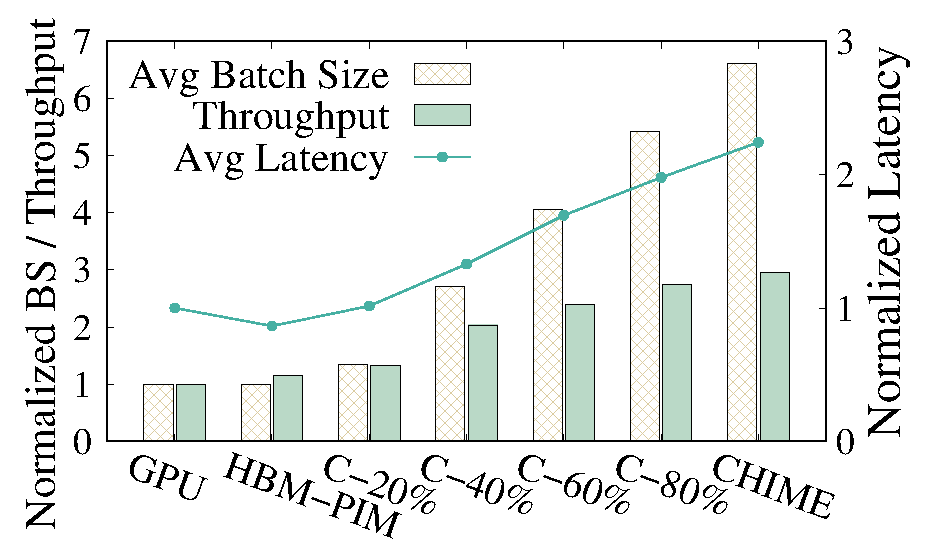
\includegraphics[width=\textwidth]{figs-eval/eval-breakdown-gpt175b.eps}
      \footnotesize
      \textbf{(a) GPT-175B.}
  \end{minipage}
  \begin{minipage}[t]{0.49\linewidth}
      \centering
      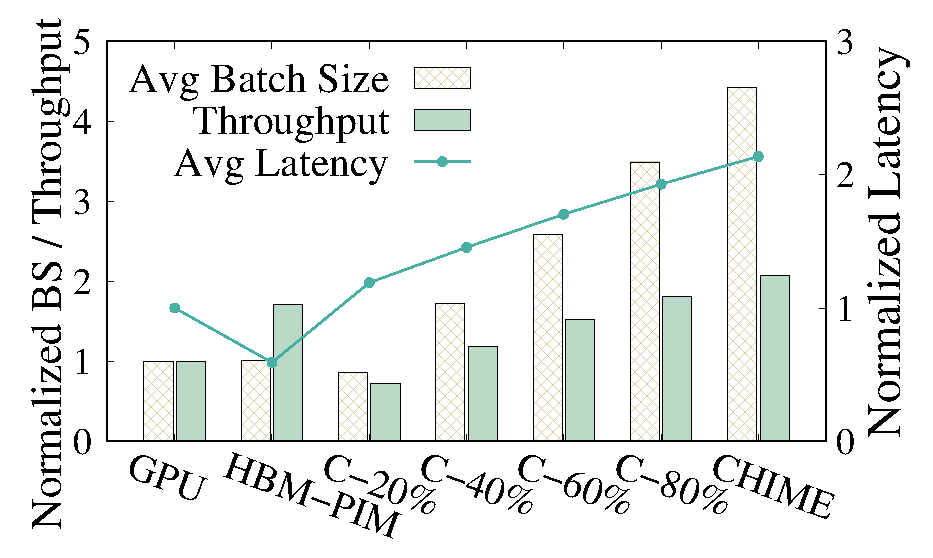
\includegraphics[width=\textwidth]{figs-eval/eval-breakdown-qwen72b.eps}
      \footnotesize
      \textbf{(b) QWEN-72B.}
  \end{minipage}
  \caption{\textbf{\REVISE{Breakdown of performance improvement with \sys.}}
      \textit{\REVISE{The results are evaluated using the OpenR1 trace. ``C-N\%'' denotes \sys with N\% available memory capacity. ``BS'' denotes ``batch size''. ``Latency'' is ``latency per batch''. The results of GPU baseline are normalized to 1}}
  } 
  \label{figs:eval-breakdown}
\end{figure}


\myparagraph{Performance improvement breakdown.}
\REVISE{
We analyze the sources of performance improvement compared with the GPU and HBM-PIM baselines. 
Fig.\ref{figs:eval-breakdown} shows the throughput, 
average batch size (the sum of two sub-batches), 
and average latency per batch from our end-to-end evaluation. 
Compared with GPU and HBM-PIM, 
\sys increases the batch size by 6.6$\times$, 
while the latency per batch increases by only $2.2\times$. 
This indicates that the throughput improvement of \sys primarily stems from the increased batch size and the corresponding improvement in GPU utilization.
}

\REVISE{
In addition, Fig.~\ref{figs:eval-breakdown} illustrates the trend of how batch size growth affects throughput. 
We manually limit the memory capacity available to \sys and measure the resulting performance. 
As the available memory gradually increases from 10\% to 100\%, 
the batch size scales linearly. 
However, since the latency per batch also increases, the rate of throughput improvement gradually diminishes. 
This observation is consistent with the analysis in Fig.~\ref{fig:intro-motiv}, 
which shows that the marginal benefit of increasing batch size on throughput decreases.
}

\myparagraph{Performance in short context scenarios.}
\REVISE{
As shown in Fig.~\ref{figs:eval-end-to-end-throughput}-d, 
in the short context scenario, 
\sys still achieves higher throughput than both the GPU and HBM-PIM baselines by achieving higher batch sizes. 
However, 
compared to Fig.~\ref{figs:eval-end-to-end-throughput}-c, 
the advantage of \sys on each model is diminished. 
This is because in the short context scenario, 
the marginal benefit of increasing the batch size exhibits diminishing returns. 
This observation is also consistent with our analysis in \textsection\ref{sec:motiv-discussion-scenarios}.
}


\begin{figure}[tb]
  \setlength{\belowcaptionskip}{-5pt}
    \begin{minipage}[t]{0.49\linewidth}
        \centering
        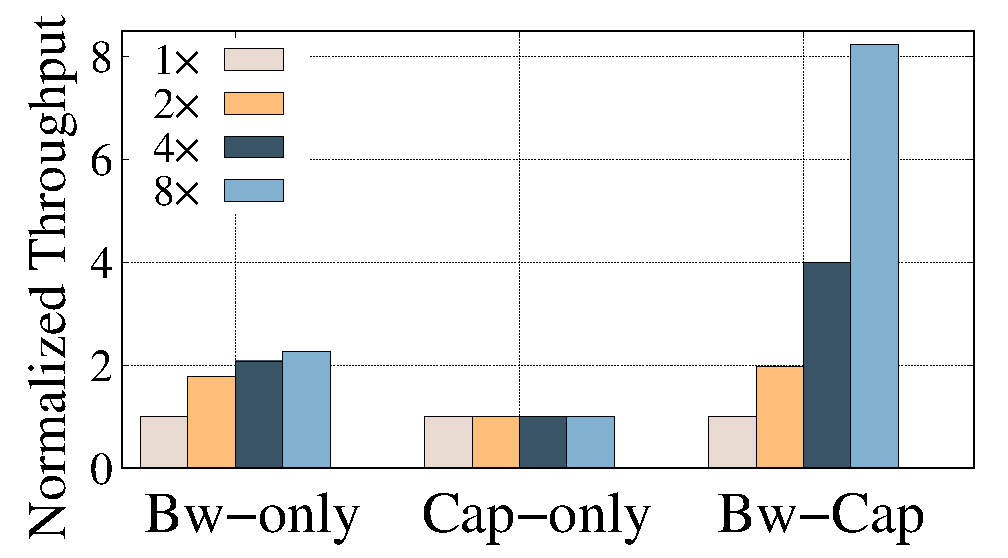
\includegraphics[width=\textwidth]{figs-eval/eval-scalability-175B-openr1.eps}
        \footnotesize
        \textbf{(a) GPT-175B.}
    \end{minipage} 
  \begin{minipage}[t]{0.49\linewidth}
    \centering
    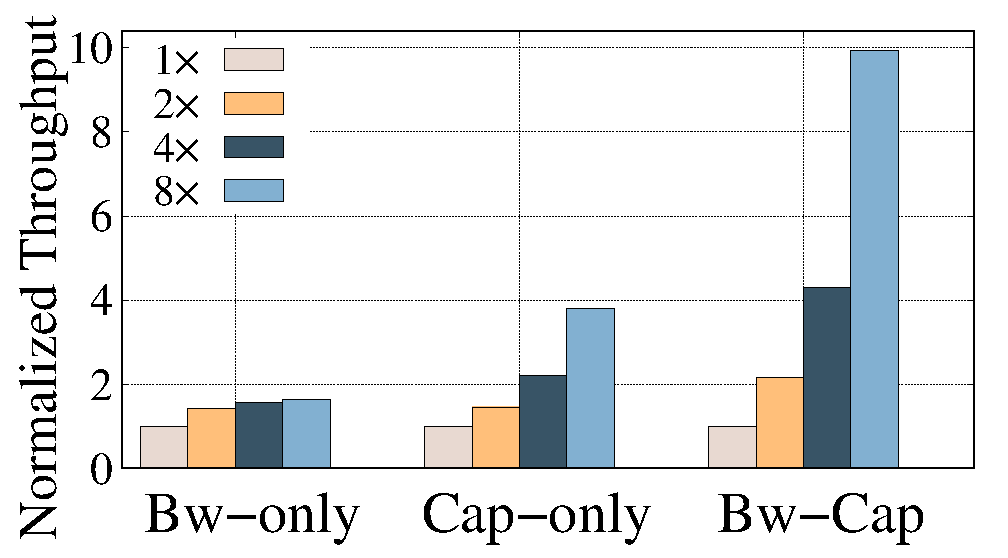
\includegraphics[width=\textwidth]{figs-eval/eval-scalability-GQA-openr1.eps}
    \footnotesize
    \textbf{(b) QWEN-72B.}
  \end{minipage} 
  \caption{\textbf{Scalability analysis.} \normalfont{\textit{The results are evaluated using the OpenR1 trace. The performance of the base memory configuration is normalized to 1.}}}
    \label{figs:eval-scalability-analysis}
  \end{figure}
  
\myparagraph{Scalability analysis.}
We further evaluate \sys performance with various \sys-PIM configurations, 
showing that performance scalability requires simultaneous scaling in memory capacity and bandwidth.
We first establish the base memory configuration as ``1 rankset, 512 GB''. 
Based on this, we scale up the memory in different ways for different baselines:
``Bw-only'' indicates that we only scale up the memory bandwidth with more ranksets but keep the capacity at 512GB, while ``Cap-only'' means we only scale up the capacity from 512GB to 4TB. 
``Bw-Cap'' implies that we scale up both the bandwidth and capacity.
We execute 1,000 requests from the trace and calculate the average throughput.

Fig.~\ref{figs:eval-scalability-analysis} shows the results of GPT-175B and QWEN-72B with OpenR1 trace. 
Results for other models and traces are similar.
It shows that expanding either bandwidth or capacity alone does not effectively improve throughput.
For example, when exclusively scaling memory capacity or bandwidth by 8$\times$ on GPT-175B, 
the throughput only increases by 2.28$\times$ and 1.01$\times$, respectively.
In contrast, when both bandwidth and capacity are enlarged, the throughput increases by 8.23$\times$. 
This demonstrates that \sys effectively leverages the value of both scalability aspects.














\begin{figure}[t]
\setlength{\abovecaptionskip}{1pt}
\setlength{\belowcaptionskip}{-5pt}
  \begin{minipage}[t]{0.49\linewidth}
      \centering
      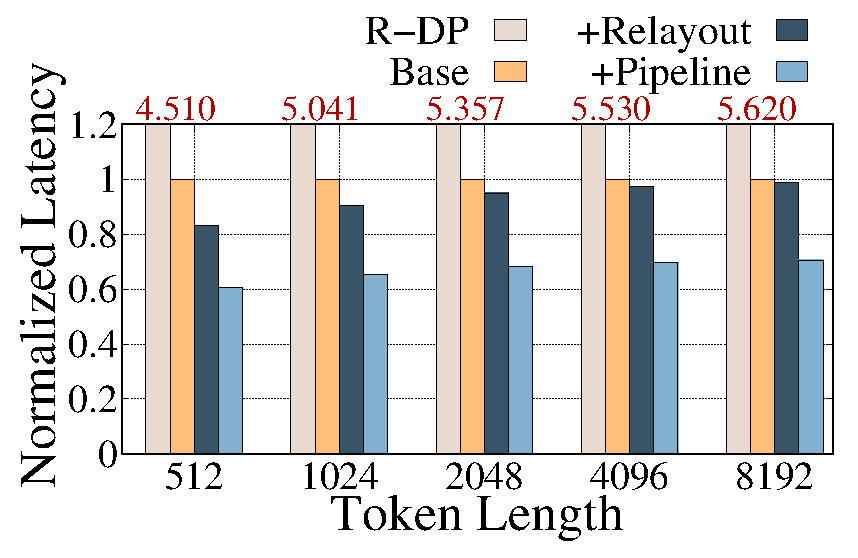
\includegraphics[width=\textwidth]{figs-eval/eval-hardware-ablation-MHA.eps}
      \footnotesize
      \textbf{(a) MHA.}
      \end{minipage}
      \begin{minipage}[t]{0.49\linewidth}
        \centering
        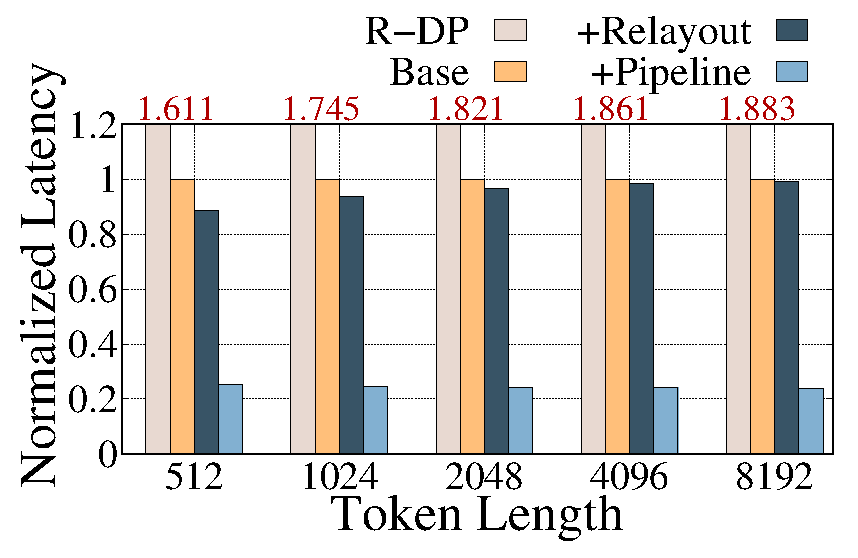
\includegraphics[width=\textwidth]{figs-eval/eval-hardware-ablation-GQA.eps}
        \footnotesize
        \textbf{(b) GQA.}
      \end{minipage}
  \caption{\textbf{Hardware ablation study.} \textit{The latency of \sys's naive implementation is normalized to 1.}} 
  \label{figs:eval-hardware-ablation}
\end{figure}



\subsection{Ablation Study}
\label{sec:eval-ablation}
\myparagraph{Ablation study for \sys-PIM.}
We analyze our hardware optimizations for: (1) bubble-free pipelining (\textsection\ref{sec:design-dp-pipeline}); (2) hybrid re-layout (\textsection\ref{sec:design-dp-relayout}). 
We implement a baseline bank-level \sys-PIM that maps head computation across chips.
Following prior work\cite{seo2025facil}, we conservatively estimate the CPU-side re-layout cost as the memory access time required to read data stored with one layout and write it into another layout.
Performance results with various token lengths are shown in Fig.~\ref{figs:eval-hardware-ablation}.
First, the bubble-free pipelining achieves about 27.9\% and 74.4\% latency reduction on MHA and GQA computation, respectively,
which is attributed to the overlapping and specific head mapping methods.
Second, the hardware hybrid re-layout enables up to 17\% latency reduction.
The reason why the proportion of gain decreases as token length increases is that the attention computation gradually dominates the overall execution time.
Nonetheless, we identify that it is still needed since the re-layout overheads accumulate in each layer of each token generation.
With all hardware optimizations, \syscolor shows 1.42--4.18$\times$ speedup. 
In addition, all bank-level implementations achieve over 1.5$\times$ speedup than the rank-level DIMM-PIM (R-DP).



\begin{figure}[t]
  \setlength{\abovecaptionskip}{0.5pt}
  \setlength{\belowcaptionskip}{-5pt}
  \begin{minipage}[t]{0.49\linewidth}
      \centering
      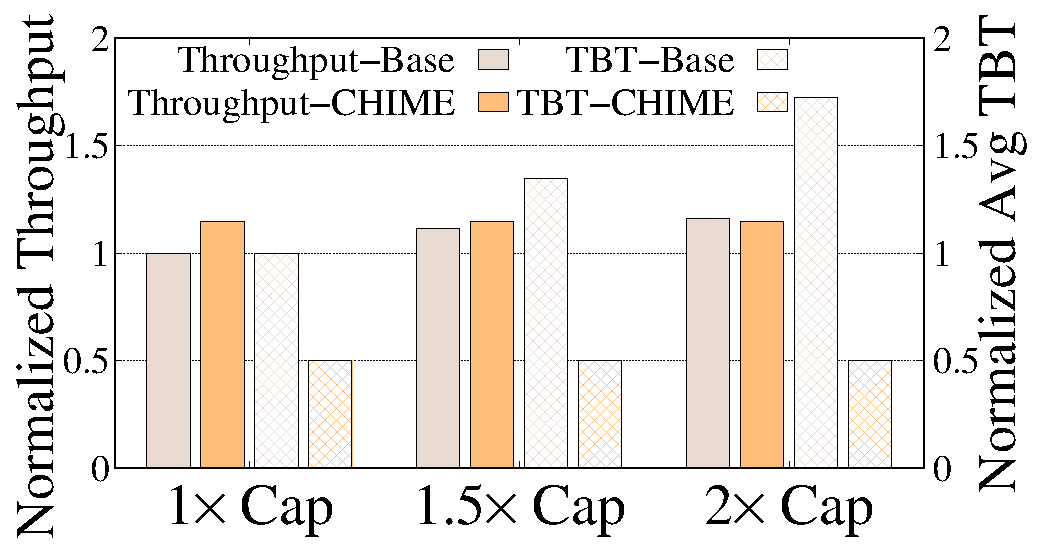
\includegraphics[width=\textwidth]{figs-eval/eval-request-select-mha.eps}
      \footnotesize
      \textbf{(a) GPT-175B.}
      \end{minipage}
      \begin{minipage}[t]{0.49\linewidth}
        \centering
        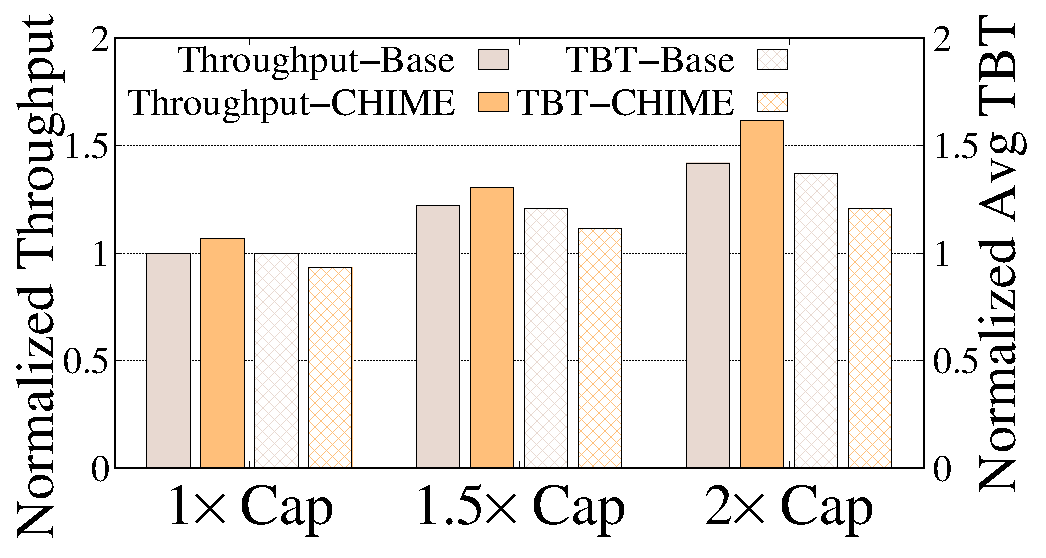
\includegraphics[width=\textwidth]{figs-eval/eval-request-select-gqa.eps}
        \footnotesize
        \textbf{(b) QWEN-72B.}
      \end{minipage}
  \caption{\textbf{Improved resource efficiency with \sys-sys.} 
      \textit{``1$\times$ Cap'' denotes the basic memory capacity (2TB for GPT-175B and 1TB for QWEN-72B) according to Table~\ref{tab:model}. 
      The results are evaluated using the OpenR1 trace.}
  } 
  \label{figs:eval-scheduler}
\end{figure}



\myparagraph{Ablation study for scheduler.}
We evaluate how \sys's scheduler effectively improves the resource utilization.
Fig.~\ref{figs:eval-scheduler} shows the average throughput and Time-between-Tokens (TBTs) of different scheduling methods on the left and right y-axes, respectively. 
The baseline represents the scheduling policy that prioritizes filling the capacity of \sys-PIM, 
while \sys denotes the alignment-predicting scheduling. 
The results show that \sys's scheduler can significantly reduce latency by up to 70.93\% without sacrificing the throughput, 
showing its ability of eliminating idle bubbles on the GPU side.
\sys even slightly improves the throughput by aligning the batches with prefilling requests and achieving better load balancing.
Moreover, for the MHA model, if we increase the capacity of \sys-PIM, 
the baseline selects larger batch sizes and causes higher TBTs without improving the throughput (since attention becomes the bottleneck), 
while \sys can avoid generating bubbles and prevent the growth of TBT.
\sys performs better with MHA models, because with the GQA model, achieving the attention bottleneck requires selecting requests that occupy larger memory capacity, or it may not even achieve the attention bottleneck.

\begin{figure}[t]
  \setlength{\abovecaptionskip}{1pt}
  \setlength{\belowcaptionskip}{-5pt}
  \centering
    \begin{minipage}[t]{0.68\linewidth}
        \centering
        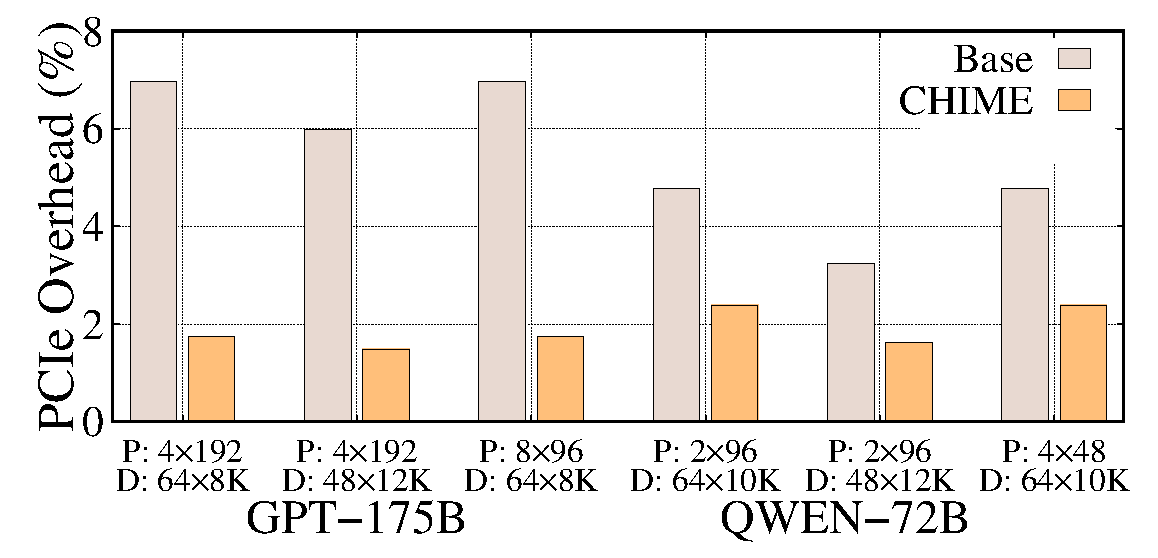
\includegraphics[width=\textwidth]{figs-eval/eval-pcie-latency-percentage.eps}
        \textbf{(a) PCIe overhead.}
        \footnotesize
    \end{minipage}
    \begin{minipage}[t]{0.30\linewidth}
        \centering
        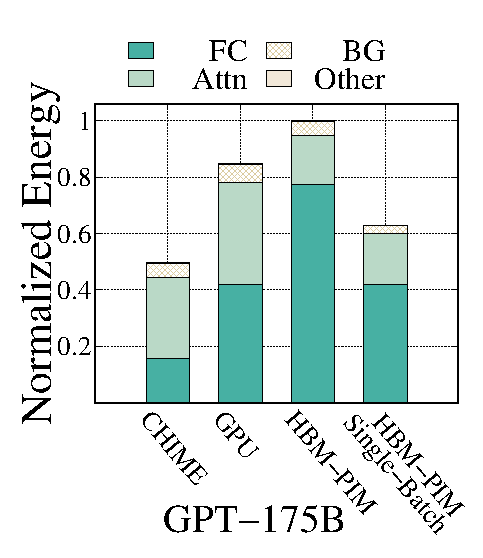
\includegraphics[width=\textwidth]{figs-eval/eval-energy-full-trace.eps}
        \textbf{\REVISE{(b) Energy.}}
        \footnotesize
    \end{minipage}
  \caption{\textbf{PCIe overhead and energy consumption.}
        \textit{``P'' and ``D'' in (a) denotes the batch sizes and token lengths of prefilling and decoding requests in a batch. The energy consumption of ``GPU'' in (b) is normalized to 1.}
     }
  \label{figs:eval-pcie-energy}
\end{figure}






\myparagraph{PCIe overhead analysis.}
We evaluate how the cross-device PCIe communication degrades the throughput with or without rankset-granular communication computation overlapping.
As shown in Fig.~\ref{figs:eval-pcie-energy}, applying the optimization could reduce the overhead by up to 75.08\% with different batch configurations.
This indicates that with the 4 ranksets of DGX-A100, most PCIe overheads are hidden with independent communication and computation at the rankset granularity.

\subsection{Cost Analysis}
\myparagraph{Energy consumption.}
\REVISE{
We evaluate the energy consumption of \sys with GPU and HBM-PIM.
For GPU-side energy, we follow the evaluation methods in AttAcc simulators. 
For PIM-side energy, 
first, we use power parameters (e.g., VDD, IDD) and timing parameters (e.g., tRAS, tRP) to calculate energy of ACT, RD, WR, and so on~\cite{micronddr4power1,micronddr4power2}. 
Second, we follow the scaling methods~\cite{mike2017fgdram,park2021trim,park2024attacc} to calculate read/write energy (e.g., MAC, Load shared buffer) inside the DRAM chips (or DRAM die); 
Third, we obtain the chip I/O energy from CACTI-IO~\cite{Jouppi2012cactiio}.
We provide three baselines: GPU, HBM-PIM, and HBM-PIM without sub-batch scheduling.}

\REVISE{
Fig.~\ref{figs:eval-pcie-energy}-b details the energy breakdown for GPT-175B on openR1 traces, 
where FC and attention computations dominate. 
First, \sys achieves a ~40\% total energy reduction, 
primarily by executing FC on the GPU with larger batch sizes, which reduces the number of weight loading. 
Second, HBM-PIM with sub-batch scheduling consumes more energy, since it halves the batch size.
Third, for attention computation, \sys-PIM's multi-chip distributed computation consumes energy comparable to the GPU but higher than HBM-PIM. 
}




\myparagraph{Hardware overhead.}
\REVISE{
We evaluate the area overhead of bank PUs, whose in-DRAM-chip integration directly impacts memory capacity.
Assuming command decoding and data paths reuse existing DRAM logic, we synthesize the design using a TSMC 28nm process. 
A single bank PU and the shared buffer consume 0.0032 $mm^2$ and 0.051 $mm^2$, respectively. 
Accounting for density differences between logic and DRAM processes, we estimate that implementation in a 1z-nm DRAM node would roughly double the synthesized area. 
While efficiently supporting GQA requires scaling the bank PU proportionally, we consider this overhead highly acceptable for two reasons.
First, the massive capacity of DIMMs, effectively amortizes the area cost. 
Further, emerging 3D integration technologies can further mitigate or eliminate this die area penalty.}


\begin{figure}[t]
  \setlength{\abovecaptionskip}{2pt}
  \setlength{\belowcaptionskip}{-10pt}
  \centering
    \begin{minipage}[t]{\linewidth}
    \centering
    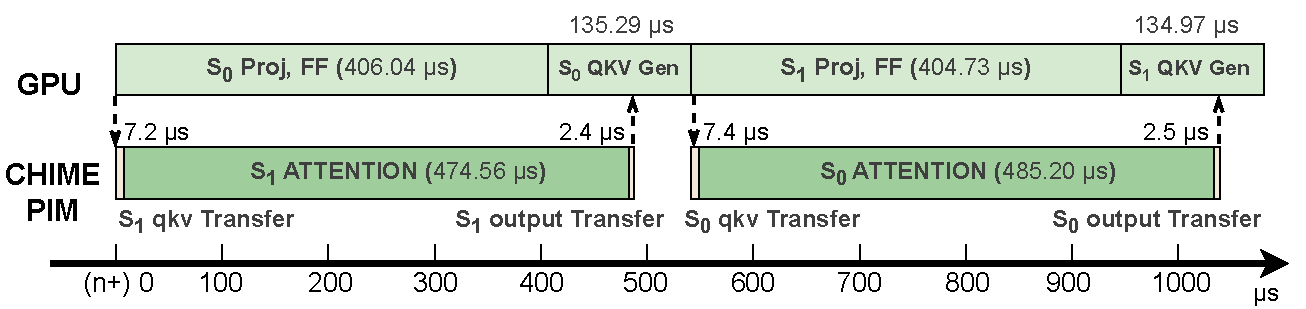
\includegraphics[width=\textwidth]{figs/pipeline-timeline.pdf}
    \footnotesize
    \end{minipage}
    \caption{\textbf{\REVISE{Decode execution timeline of CHIME pipeline for single LLM layer.}}
    \textit{\REVISE{The batch is executed with GPT-175B and the OpenR1 trace.}}}
  \label{fig:eval-pipeline-timeline}
\end{figure}

\myparagraph{Timeline breakdown analysis.}
\REVISE{
As shown in Fig.~\ref{fig:eval-pipeline-timeline}, 
we extract a representative batch from the actual execution of the end-to-end evaluation as an example and perform a detailed timeline breakdown analysis. 
We observe that with our designs, the computation on the GPU and PIM sides is effectively pipelined with minor bubbles.
}








